\subsection{State Feedback with Integral Control Design}
The aim of the controller is to be able to track a reference, within a reasonable range, in the three angles that define the attitude of the quadcopter.

Given a state space representation as the one in \autoref{xDotLinear} and \autoref{yLinear}, it is possible to design a controller so that the final dynamics of the system can be chosen.

In this approach a state feedback is used to allow the system to return to equilibrium position while a integral control makes possible to include a reference and track it, adding both control actions to get the one finally applied to the motors. The diagram in \autoref{fig:DetailedControllerColorDiagram} shows how these controllers are related.
%
\begin{minipage}{\linewidth}
	\begin{minipage}{0.6\linewidth}
		\begin{figure}[H]
			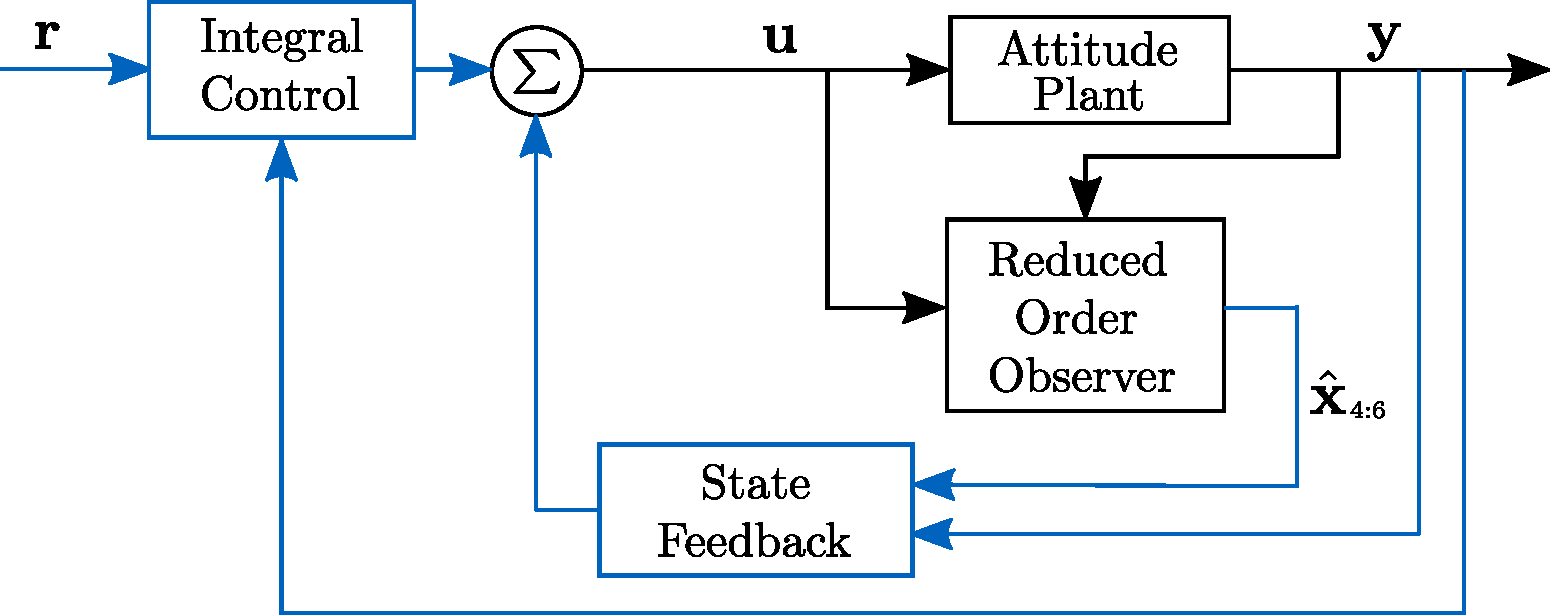
\includegraphics[scale=.35]{figures/ControllerColorDiagram}
			\centering			
			\captionof{figure}{Control structure with the state feedback and integral control parts highlighted.}
			\label{fig:ControllerColorDiagram}
		\end{figure}
	\end{minipage}
	\hspace{0.03\linewidth}
	\begin{minipage}{0.4\linewidth}
		\begin{figure}[H]\vspace{20mm}
			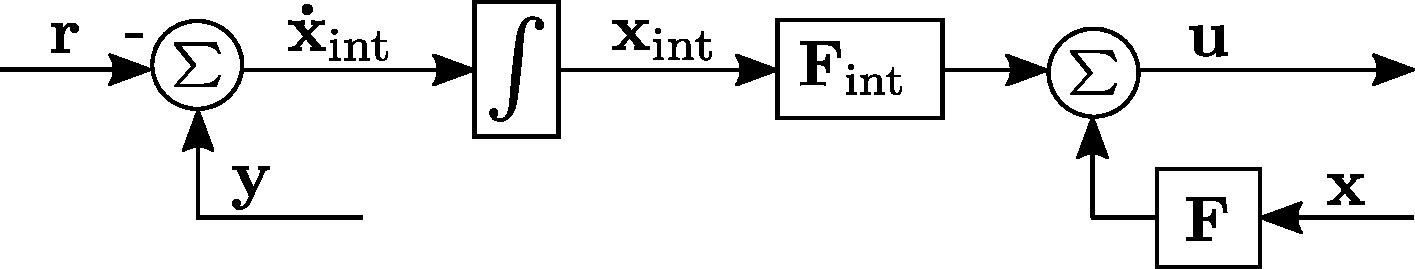
\includegraphics[scale=.35]{figures/DetailedControllerColorDiagram}
			\centering \vspace{7mm}
			\captionof{figure}{Detail of the left diagram, that includes all the variables used in the design of the controller.}
			\label{fig:DetailedControllerColorDiagram}
		\end{figure}
	\end{minipage}
\end{minipage}


The feedback law is given by \autoref{eq:ssControllerAction}.
%
\begin{align} 
	\vec{u}(t) &=\vec{F} \cdot \vec{x}(t) + \cdot\vec{F}_{Int} \cdot \vec{x}_{Int}(t)
\end{align} \label{eq:ssControllerAction}
%
\begin{where}
	\va{\vec{F}}{is the 4x6 state feedback matrix}{}
	\va{\vec{F}_{Int}}{is 3x6the asdffsfaf matrix }{}
\end{where}
%
In this equation, \si{\vec{x}_{Int}(t)} is given by \autoref{eq:ssControllerAction1}, that is equivalent to \autoref{eq:ssControllerAction2}.
\begin{flalign}
    \vec{x}_{Int}(t) &= \int_{0}^{t} \vec{y}(\tau)-\vec{r}(\tau) d\tau	\label{eq:ssControllerAction1}\\
    \vec{\dot{x}}_{Int}(t) &= \vec{y}(t)-\vec{r}(t) \label{eq:ssControllerAction2}
\end{flalign} 
%
This last equation can be introduced in the existing state space model, taking \si{\vec{x}_{Int}(t)} as new states, and giving the result shown in \autoref{xdotSSExtended} and \autoref{ySSExtended}.
%
\begin{flalign} 
    \dot{\vec{x}}_e(t) &= \vec{A}_e \cdot \vec{x}_e(t) + \vec{B}_e \cdot \vec{u}(t) + 
    \begin{bmatrix}
       \ 0     \ \ \ \\ 
       \ \vec{-I}     \ \ \  		
   \end{bmatrix}
   \vec{r}(t) 
   \label{xdotSSExtended}\\ 
    \vec{y}(t) &= \vec{C}_e \cdot \vec{x}_e 
       \label{ySSExtended}
\end{flalign} 
%
being\\
\begin{minipage}{0.24\linewidth}
	\begin{flalign}
		\dot{\vec{x}}_e(t)= 
		\begin{bmatrix}
			\ \dot{\vec{x}}(t)      \ \ \ \\ 
			\ \dot{\vec{x}}_{Int}(t)      \ \ \  		
		\end{bmatrix} \nonumber
	\end{flalign}
\end{minipage}\hfill
\begin{minipage}{0.24\linewidth}
	\begin{flalign}
	    \vec{A}_e=
	    \begin{bmatrix}
	        \ \vec{A}  & 0    \ \ \ \\ 
	        \ \vec{C}  & 0    \ \ \  		
	    \end{bmatrix} \nonumber
	\end{flalign}
\end{minipage}   \hfill 
\begin{minipage}{0.24\linewidth}
	\begin{flalign}
		\vec{B}_e=
		\begin{bmatrix}
			\ \vec{B}    \ \ \ \\ 
			\ 0     \ \ \  		
		\end{bmatrix} \nonumber
	\end{flalign}
\end{minipage}\hfill
\begin{minipage}{0.24\linewidth}
	\begin{flalign}
		\vec{C}_e=
		\begin{bmatrix}
			\ \vec{C}  & 0  \ \ \  		
		\end{bmatrix} \nonumber
	\end{flalign}
\end{minipage}

The resulting feedback law can be design as a conventional state feedback, where the goal is to choose an appropriate $F_e=[F \ F_{Int}]$ matrix such that the eigenvalues of $A_e+B_eF_e$ are the new poles that the system needed to have in order to achieve the desired dynamics.

Once $F_e$ is obtained, it can be slitted into $F$ and $F_{Int}$ by taking the first 6 columns for the state feedback and the last 3 for the integral control. In this way, the controller can be implemented as shown in \autoref{fig:DetailedControllerColorDiagram}





